\section{一种新的单细胞稀有细胞及类型识别方法}

基于液滴~(drop)的转录组学技术的出现,平台已经实现了对数千或数百万细胞的并发筛选。
其中一个具有挑战性的问题是如何从超大规模的~scRNA-seq~数据中识别稀有细胞及其类型。
现有的寻找稀有细胞的算法非常耗时或耗费内存。
本文中,我们提出了一种高效准确的方法~DoRC~(\underline{D}iscovery \underline{o}f \underline{R}are \underline{C}ells)。
DoRC~产生的稀有度分数可以帮助生物学家们着重于下游分析,只对超大规模内的部分表达细胞~scRNA-seq~数据进行分析。
为了在随后的下游分析的过程中区分细胞类型,我们提出了新颖有效的细胞聚类方法~RafClust。
我们使用~${\sim}68$k~人血细胞的单细胞表达谱还证明了~DoRC~在划分人类血液树突状细胞亚型方面的效果。
DoRC可以识别仿真数据集里面的稀有细胞,并且对细胞类型特征也很敏感。

\subsection{介绍}
单细胞~RNA-seq~(scRNA-seq)~技术提供了单细胞水平的转录组测量。
使不同组织中细胞类型的鉴定和表示成为可能。
相比之下,传统的批量~RNA~测序的表达值是数千或数百万细胞的平均值,因此存在局限性。
scRNA-seq~技术的出现提供了一个从细胞水平研究生物机制的前所未有的视角,
使得研究人员更严格地处理一些生物问题,比如组织的细胞组成、转录组的异质性,
以及细胞在发育过程中或在疾病和癌症中类型是如何变化~\cite{kumar2017understanding,patel2014single}。

scRNA-seq技术的一个非常迫切和具有挑战性的应用,是从组织中的一堆细胞中捕获稀有细胞。
稀有细胞代表了生物体内的次要细胞类型,当测序细胞的数量在数百个规模时,即使是一个孤立的离群点~(singleton)~也值得关注。
然而,随着吞吐能力的提高,研究重点转换到次要细胞类型的发现,再也不仅仅是单纯的单个细胞。
稀有细胞类型包括循环肿瘤细胞、癌症干细胞、循环内皮细胞、内皮祖细胞、抗原特异性T细胞、不变性自然杀伤性T细胞等。
尽管丰度较低,但稀有细胞群在决定癌症的发病机制、介导免疫反应、癌症和其他疾病的血管生成等方面起着核心作用。
抗原特异性T细胞对免疫学记忆的形成至关重要~\cite{slansky2003antigen,altman1996phenotypic,manzo2015antigen}。
内皮祖细胞,来源于骨髓,已被证明是肿瘤血管生成的可靠生物标志物~\cite{kuo2012dynamics,cima2016tumor}。
干细胞可以替代受损细胞,并用于治疗帕金森氏症、糖尿病、心脏病等疾病~\cite{jang2005stem}。
循环肿瘤细胞提供了前所未有的洞察力,为临床管理提供了实时线索~\cite{krebs2010circulating}。

由于最近发现了基于液滴的单细胞转录组学,使得数以万计的单细胞的并行测序成为可能。
单个细胞的测序成本显著降低的情况下,稀有细胞的鉴别也变为可行。
迄今为止,已经有许多研究发表了使用的转录组,细胞数量范围在~${\sim} 20$k和~${\sim} 70$k~之间。
大的转录组样本量通过削弱由于扩增阶段的失败所带来的影响,可以更好地捕捉到组织中的微小细胞亚群。
事实上,稀有细胞检测已经成为目前下游分析流程中的不可缺少的一环。

到目前为止,聚焦于研究怎样去检测稀有细胞转录组的算法还很少。
其中突出的方法有~RaceID~\cite{grun2015single},GiniClust~\cite{jiang2016giniclust}和FiRE~\cite{jindal2018discovery}。
RaceID~涉及到计算昂贵的参数模型,并用于检测离群的表达谱值。
它使用了\textit{k}-means聚类这种典型的基于距离的方法和间隙统计计算,
作为识别大量细胞类型的中间步骤,
这些数据又反过来辅助确定离群事件~(基因)。
另一方面,~GiniClust~使用了一个相当直接的双管齐下的算法。
它首先使用~Gini~指数选择信息量大的基因,
然后它应用基于密度的空间聚类应用与噪声~(DBSCAN)~\cite{ester1996density},来发现离群细胞。
值得注意的是,~RaceID~和~GiniClust~都使用聚类来区分主要和次要细胞类型之间。
对于超大的~scRNA-seq~数据来说,速度非常慢,而且内存使用效率低。
相比之下,~FiRE~为研究中的每一个细胞表达谱计算出一个稀有度分数。
它使用~Sketching~技术~\cite{wang2007sizing}来估计每个细胞的密度,
对于大量数据点的低维编码来说,FiRE~是非常强大的。
对于大量的~scRNA-seq~数据,FiRE~的运行时间效率令人印象深刻。

我们提出了~DoRC,
从超大规模~scRNA-seq~数据中快速检测稀有细胞的方法。
DoRC~的设计灵感来自于对稀有度估计的观察。
多维空间中某一特定点,可以看作是机器学习中的异常检测问题。
据我们所知,DoRC~是第一个从超大规模~scRNA-seq~数据中发现稀有细胞的异常检测方法。
在~DoRC~中,每个细胞的稀有度用每个给定点的``异常得分"来表示。
这是通过使用孤立森林~\cite{liu2008isolation}实现的。
我们在多个真实和模拟数据集上对~DoRC~进行了评估。
我们展示了~DoRC~在使用~${\sim}68$k~这个人血细胞的单细胞表达谱来划分人血树枝状细胞亚型。
此外,在其他两个模拟数据集上的实验显示~DoRC~可以识别仿真数据集中的稀有细胞,
并且对细胞类型特征也很敏感。
我们对该方法的测试实验还表明,~DoRC~是快速可扩展的的。

\subsection{数据集和方法}
\label{sec:method}

\subsubsection{数据集描述}
\label{subsec:datasets} 
第一个数据集\textit{PBMCs\_68k}由~68579~个从健康供体收集的~PBMCs~组成~\cite{zheng2017massively}。
11~个纯化的~PBMCs~亚群的单细胞表达谱被用作细胞类型注释的参考。
该数据集可在~\url{www.10xgenomics.com}。

%第二个数据集textit{MSE/20k}包含了来自小鼠大脑Arc-ME区域周围的~${sim} 20$k scRNA-seq图谱~\cite{campbell2017molecular}。
%作者将神经元细胞分为34个簇。
%和非神经元细胞通过二传聚类方法分为30个聚类。
%我们只关注30个非神经元集群,其中包括8092个非神经元细胞。
%数据集~(GSE93374)~是从\url{https://hemberg-lab.github.io/scRNA.seq.datasets/mouse/brain/}下载的。

第二个数据集~\textit{Jurkat\_293T}是由~Jurkat和~293T的两个表达谱构建的,同样来自同一研究~\cite{zheng2017massively}。
Jurkat数据集由~3258~个细胞组成,而~293T~数据集由~2885~个细胞组成。
首先,从~293T~数据集中不放回抽样~1500~个细胞。
然后,通过从~Jurkat~数据集中取样不同数量的细胞,
产生~8~个数据集,其中~Jurkat~细胞数分别为0.5\%、1\%、1.5\%、2\%、2.5\%、5\%、10\%、15\%。
这两个数据集的表达矩阵也可以从~\url{www.10xgenomics.com}下载。

最后一个数据集~\textit{Splatter\_500}是一个人工仿真~scRNA-seq~数据,
通过使用\textit{splatter} R~包~\cite{zappia2017splatter},由~500~个细胞组成。
与两种细胞类型:25~个细胞是罕见的,其他~475~个细胞是丰富的。
在这个数据集中,每个细胞有~5000~个基因。
使用下面的命令来生成这个数据集:

\texttt{splatSimulate(group.prob = c(0.95, 0.05), method = groups, 
verbose = F, batchCells = 500, de.prob = c(0.4, 0.4), out.prob = 0, 
de.facLoc = 0.4, de.facScale = 0.8, nGenes = 5000)}

\subsubsection{DoRC方法}
DoRC~方法是用于从超大型~scRNA-seq~数据中发现稀有细胞,包括几个子步骤,如图~\ref{fig:flowchart}~所示。
所有子程序的细节在下文中详述。
\begin{figure}[!htbp]
    \centering
    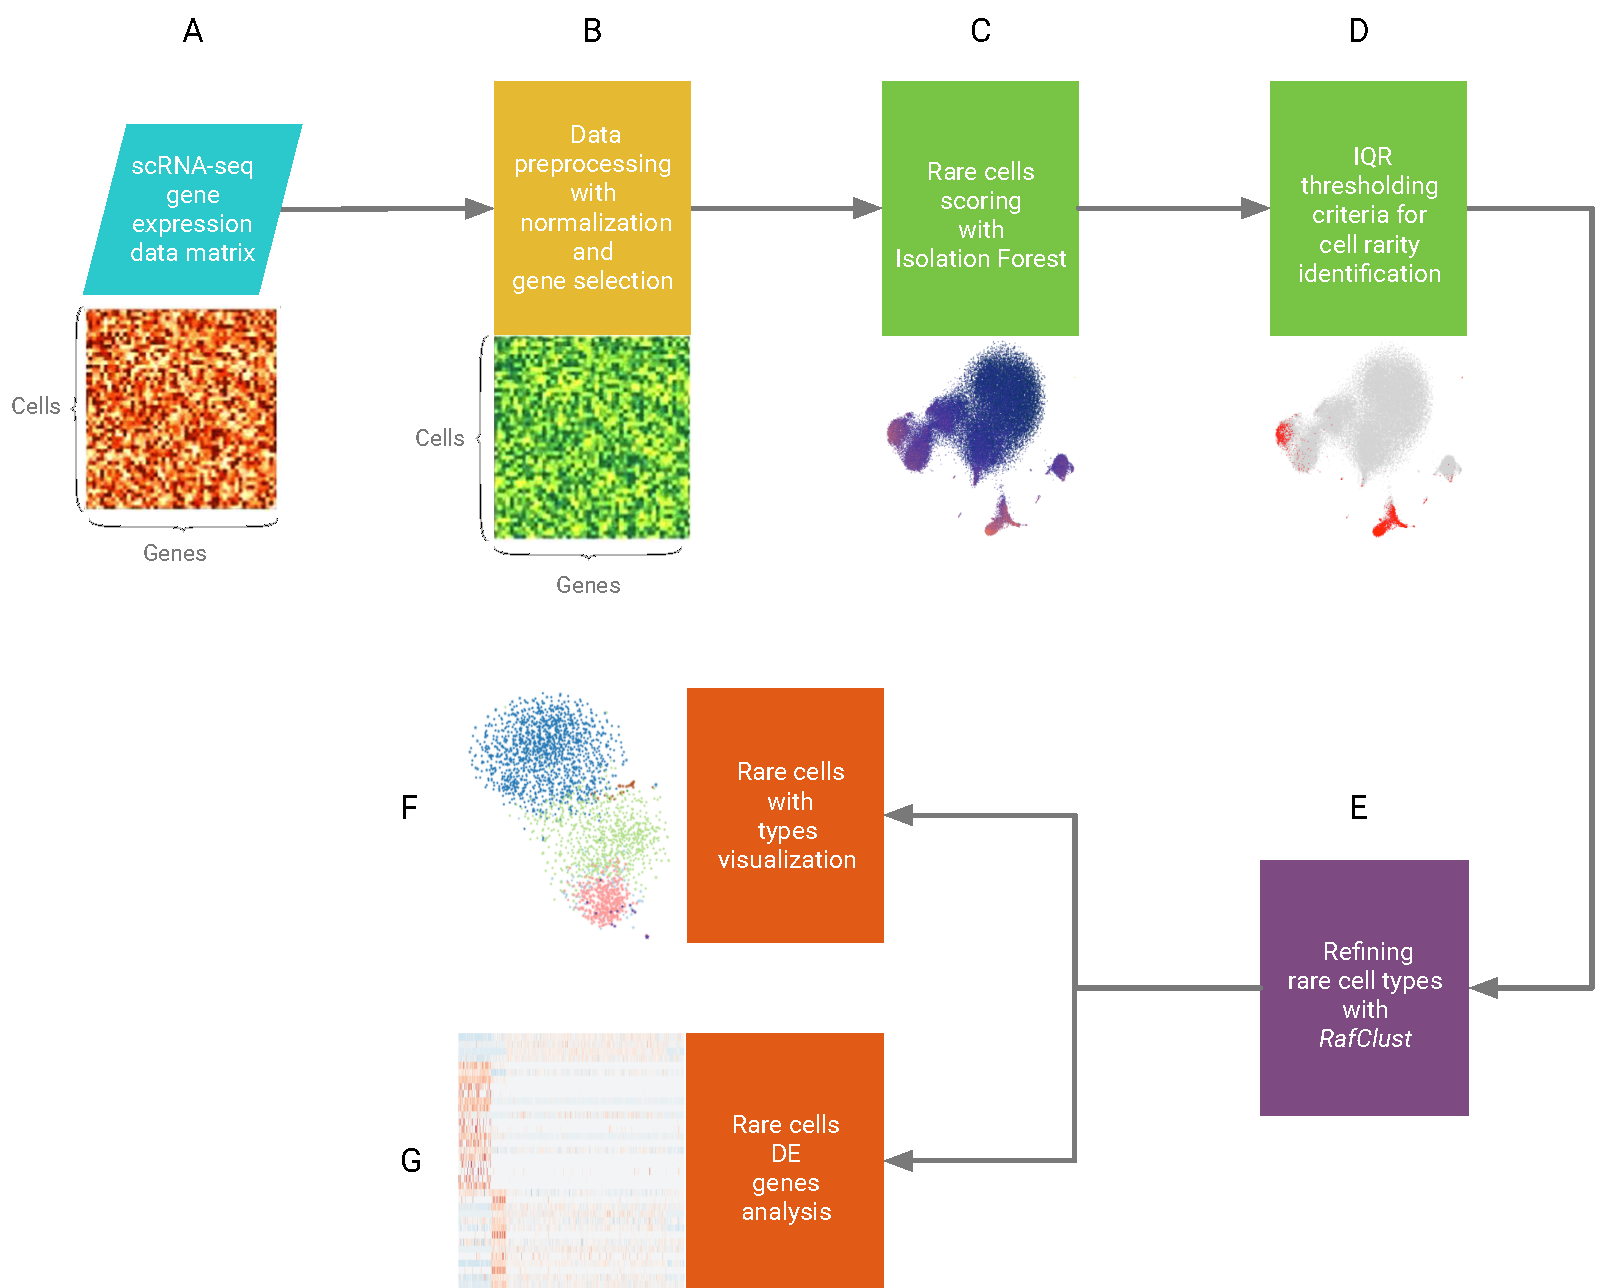
\includegraphics[width=0.95\textwidth]{flowchartv4.pdf}
    \caption{DoRC flowchart. The flowchart illustrates the processes of our proposed DoRC method for rare cells detection from ultra-large scRNA-seq data. 
    Each annotated vignette in this figure represents the input or output visualization for the corresponding procedure. 
    (A) The input is the scRNA-seq expression data 2D-matrix, whose row stands for cells, column for genes, respectively.
    (B) Data preprocessing with the input expression data, the output is  a normalized and the column dimension reduced matrix. 
    (C-D) Rare cells discovery with Isolation Forest, which are the workhorse procedures of DoRC. 
    (C) Rare cells scoring with Isolation Forest, the output is a list of continuous anomaly scores for all the cells.
    The scores can be visualized in the t-SNE-based 2D plot of the dataset; 
    (D) IQR thresholding criteria for cell rarity identification, the binary annotations are also visualized in the t-SNE-based 2D plot.
    (E) Refining rare cell types with RafClust. Notably, this sub-procedure is optional if we do not care about the types of rare cells.
    (F) Rare cells with types visualization, different colors represent different rare cell types in the t-SNE-based 2D plot of the rare cells.
    (G) Different expression genes analysis with different types of rare cells, the cell type specific genes are consequently obtained. 
    }
    \label{fig:flowchart}
\end{figure}

\subsubsection{数据规范化和基因选择}
\label{subsec:datapreprocessing} 
每个数据集上,在至少~3~个细胞中读数超过~2~的基因被保留用于下游分析,
然后使用中位数归一化。
除~\textit{Splatter\_500}~之外的其它数据集,
我们基于基于它们的相对分散度(方差/均值)与具有相似平均表达量的基因之间的预期分散度~\cite{zheng2017massively,macosko2015highly}选出~1000个变化最大的基因。
最后,将处理后的伪数矩阵加~1~后进行对数变换。

\subsubsection{使用孤立森林识别稀有细胞}
\label{subsec:if} 

孤立森林是一种无模型算法,它的计算效率很高,非常适合并行计算方法的使用~\cite{hariri2018batch}。
事实证明,它在检测异常方面也是非常有效的~\cite{susto2017anomaly}。
该算法的主要优越性在于,它并不依赖于为数据设置一个配置文件,以寻找不严格匹配该配置文件的样本。
相反,它利用了异常数据``少而不同"的特点。
其他大多数异常检测算法都是通过了解异常数据的属性分布,并将其从其他正常数据样本中分离出来,从而找到异常数据~\cite{noto2010anomaly,chen2011ordinal,das2016incorporating}。
在孤立森林中结合树结构,从数据中抽取子样本,
并根据数据集中随机选取的特征值进行随机切割。
树枝路径越长,那么该样本为异常样本的可能性越低;
相反,路径越短的树枝越有可能是异常的。
因此,每个树枝的总长度可以被看作是对指定点的异常性衡量的``异常得分"。

孤立森林~\cite{liu2008isolation,liu2012isolation}~的算法思想同任何基于树结构的聚合方法一样,
也是在基于决策树结构之上的。
在训练时,给定一个维度为~$N$~的数据集,
该算法选择一个随机的数据子样本来构建一棵二叉树。
树的分支过程通过选择一个随机维度~$x_i$,也就是一个单一的变量或特征来进行,其中~$i \in {1,2,\ldots,N}$。
如果一个给定的数据点在维度~$x_i$~的值小于~$v$,~$v$~是该维度中最小值和最大值内的随机值,
那么这个点就会被送到左分支;否则,就会走到右分支。
通过这种方式,树节点当前的数据被分割成两个子数据集。
这个分支过程在数据集上递归执行,直到一个点被隔离,或者达到预定的深度限制。
这个过程再次开始,用一个新的随机子样本来建立另一棵随机化树。
在建立一个大的树的集合后,也就是一片森林,训练的过程就完成了。
在评分步骤中,新的候选数据点或用于创建树的现有数据点贯穿所有树。
根据指定点在每棵树中达到的深度,聚合的异常得分的计算方法是:
\begin{equation}
    \label{as}
    s(x,n) = 2^{-E(h(x))/c(n)}
\end{equation}
其中, $E(h(x))$~是单个数据点~$x$~在所有树中达到的深度的平均值, $h(x)$~代表~$x$~在树中的深度~(高度)。 
$c(n)$~是归一化因子,定义为二叉搜索树~(BST)~中搜索失败的平均深度。
\begin{equation}
    \label{lab:as}
    c(n) = 2H(n - 1) - (2(n - 1)/n)
\end{equation}
其中~$H(i)$为谐波数,
可由~$ln(i)~+~0.5772156649$(欧拉常数)~\cite{liu2012isolation}估计,$n$~为建树时所用的点数。
$s(x,n)$的值接近~1表示异常,远小于~0.5表示正常观测值。
我们在这里使用的参数默认值与~\cite{liu2008isolation,liu2012isolation}一样,
即在所有实验中子样本数据为~256,树的集合为~100。

虽然连续的异常得分是很有帮助的,但有时关于细胞稀有度的二进制注释可以极大地简化分析管道。
因此,如果一个细胞的~DoRC~得分,即聚合异常得分,大于~$q_3 + 1.5 \times IQR$,则~DoRC将其标记为罕见,
其中~$q_3$和~$IQR$分别表示所有细胞中~DoRC~分数的第三分位数和四分位数范围(第75百分位数$-$第25百分位数)。

\subsubsection{使用~RafClust确定细胞类型}
\label{subsec:rafclust} 
为了从稀有细胞集合中确认不同的细胞类型,我们提出了一种无监督的基于随机森林的相似性学习算法,命名为~RafClust。

类似于其它的许多方法~\cite{kiselev2017sc3,pouyan2018random,mohammadi2018geometric,sinha2018dropclust,Srinivasan511626,Li530378,zheng2019sinnlrr},
RafClust~也是两个步骤的方法,
第一个步骤是我们使用随机森林进行相似度学习~(相似性学习步骤),
在第二步骤中我们使用层次聚类~(聚类步骤)。
在相似度学习步骤中,一个非常关键的预处理程序是特征矩阵的构建。
我们假设归一化的~$n$~细胞的基因表达数据~(观测值)~和~$p$~的基因(特征),
组成成一个~$n \times p$~的表达式矩阵~$X=\left(x_{1}, x_{2}, \ldots, x_{n} \right)^ T$。
其中$x_{i}$表示$p$基因在细胞$i$中的表达。
$x_{i}=\left(x_{i1}, x_{i2} ,\ldots, x_{ip} \right)$。
矩阵~$X$在加上~1的伪数后进行对数变换。
$X^{\prime} = log_2 (X + 1)$。
然后,如果基因在所有细胞中的平均累积表达量低于一个预定义的分数$\beta$,则会被删除。
默认情况下,$\beta$~设置为~0.06。 
基因过滤的动机是,除了保守的基因外,其它一些很普通的基因往往对聚类没有参考价值。
基因过滤这一步骤是可选的,如果基因本身都是高表达的,这个步骤可以跳过。
稀有细胞与丰富细胞不同,我们打算选择更多不同类型的细胞和细胞的相似性来充分刻画它们的本性特征。
因此,在基于基因过滤后的表达矩阵~$X^{\prime}$~上,
我们利用欧几里德~(Euclidean)、皮尔逊~(Pearson)~和斯皮尔曼~(Spearman)~指标分别计算出三种不同的细胞-细胞距离矩阵~$\{C_1, C_2, C_3\}$。
然后将PCA应用于每个距离矩阵,也用~$X^{\prime}$,来减少数据维度的同时也去除其本能噪声。
每个矩阵中信息量最大的成分由``elbow法''~\cite{thorndike1953belongs}保留。
这就产生了四个~$\left\{ {F}_{i} \in \mathbb {R} ^ {n \times m_{i}} \right\}_{i = 0}^{3}$~矩阵。
最终的人工指定的特征矩阵~$F$~由这些矩阵并列拼接组成。
\begin{equation}
\label{lab:f}
{F} = ({F}_{0}, {F}_{1}, {F}_{2}, {F}_{3})
\end{equation}

$F$~中的列数~(维度)~(即特征总数~$\tilde {p} = \sum_{i = 1}^{k} m_{i}$)~与数据有关。
和细胞~$j$~现在用特征向量~$f_{i} \in \mathbb {R} ^ {\tilde{p}}$~表示。
$F$~是这样得到的,对于每个细胞,
其自身表达值和与其他细胞的相似性关系都被表示出来。
接着,利用特征矩阵~$F$~来进行基于随机森林~(RF)~的相似性学习。
举一个例子,在~$15 \times 15$~基因表达矩阵的数据集上来说明整个特征矩阵的构建步骤如图~\ref{fig:rafsim}所示。
\begin{figure}[!htbp]
    \centering
    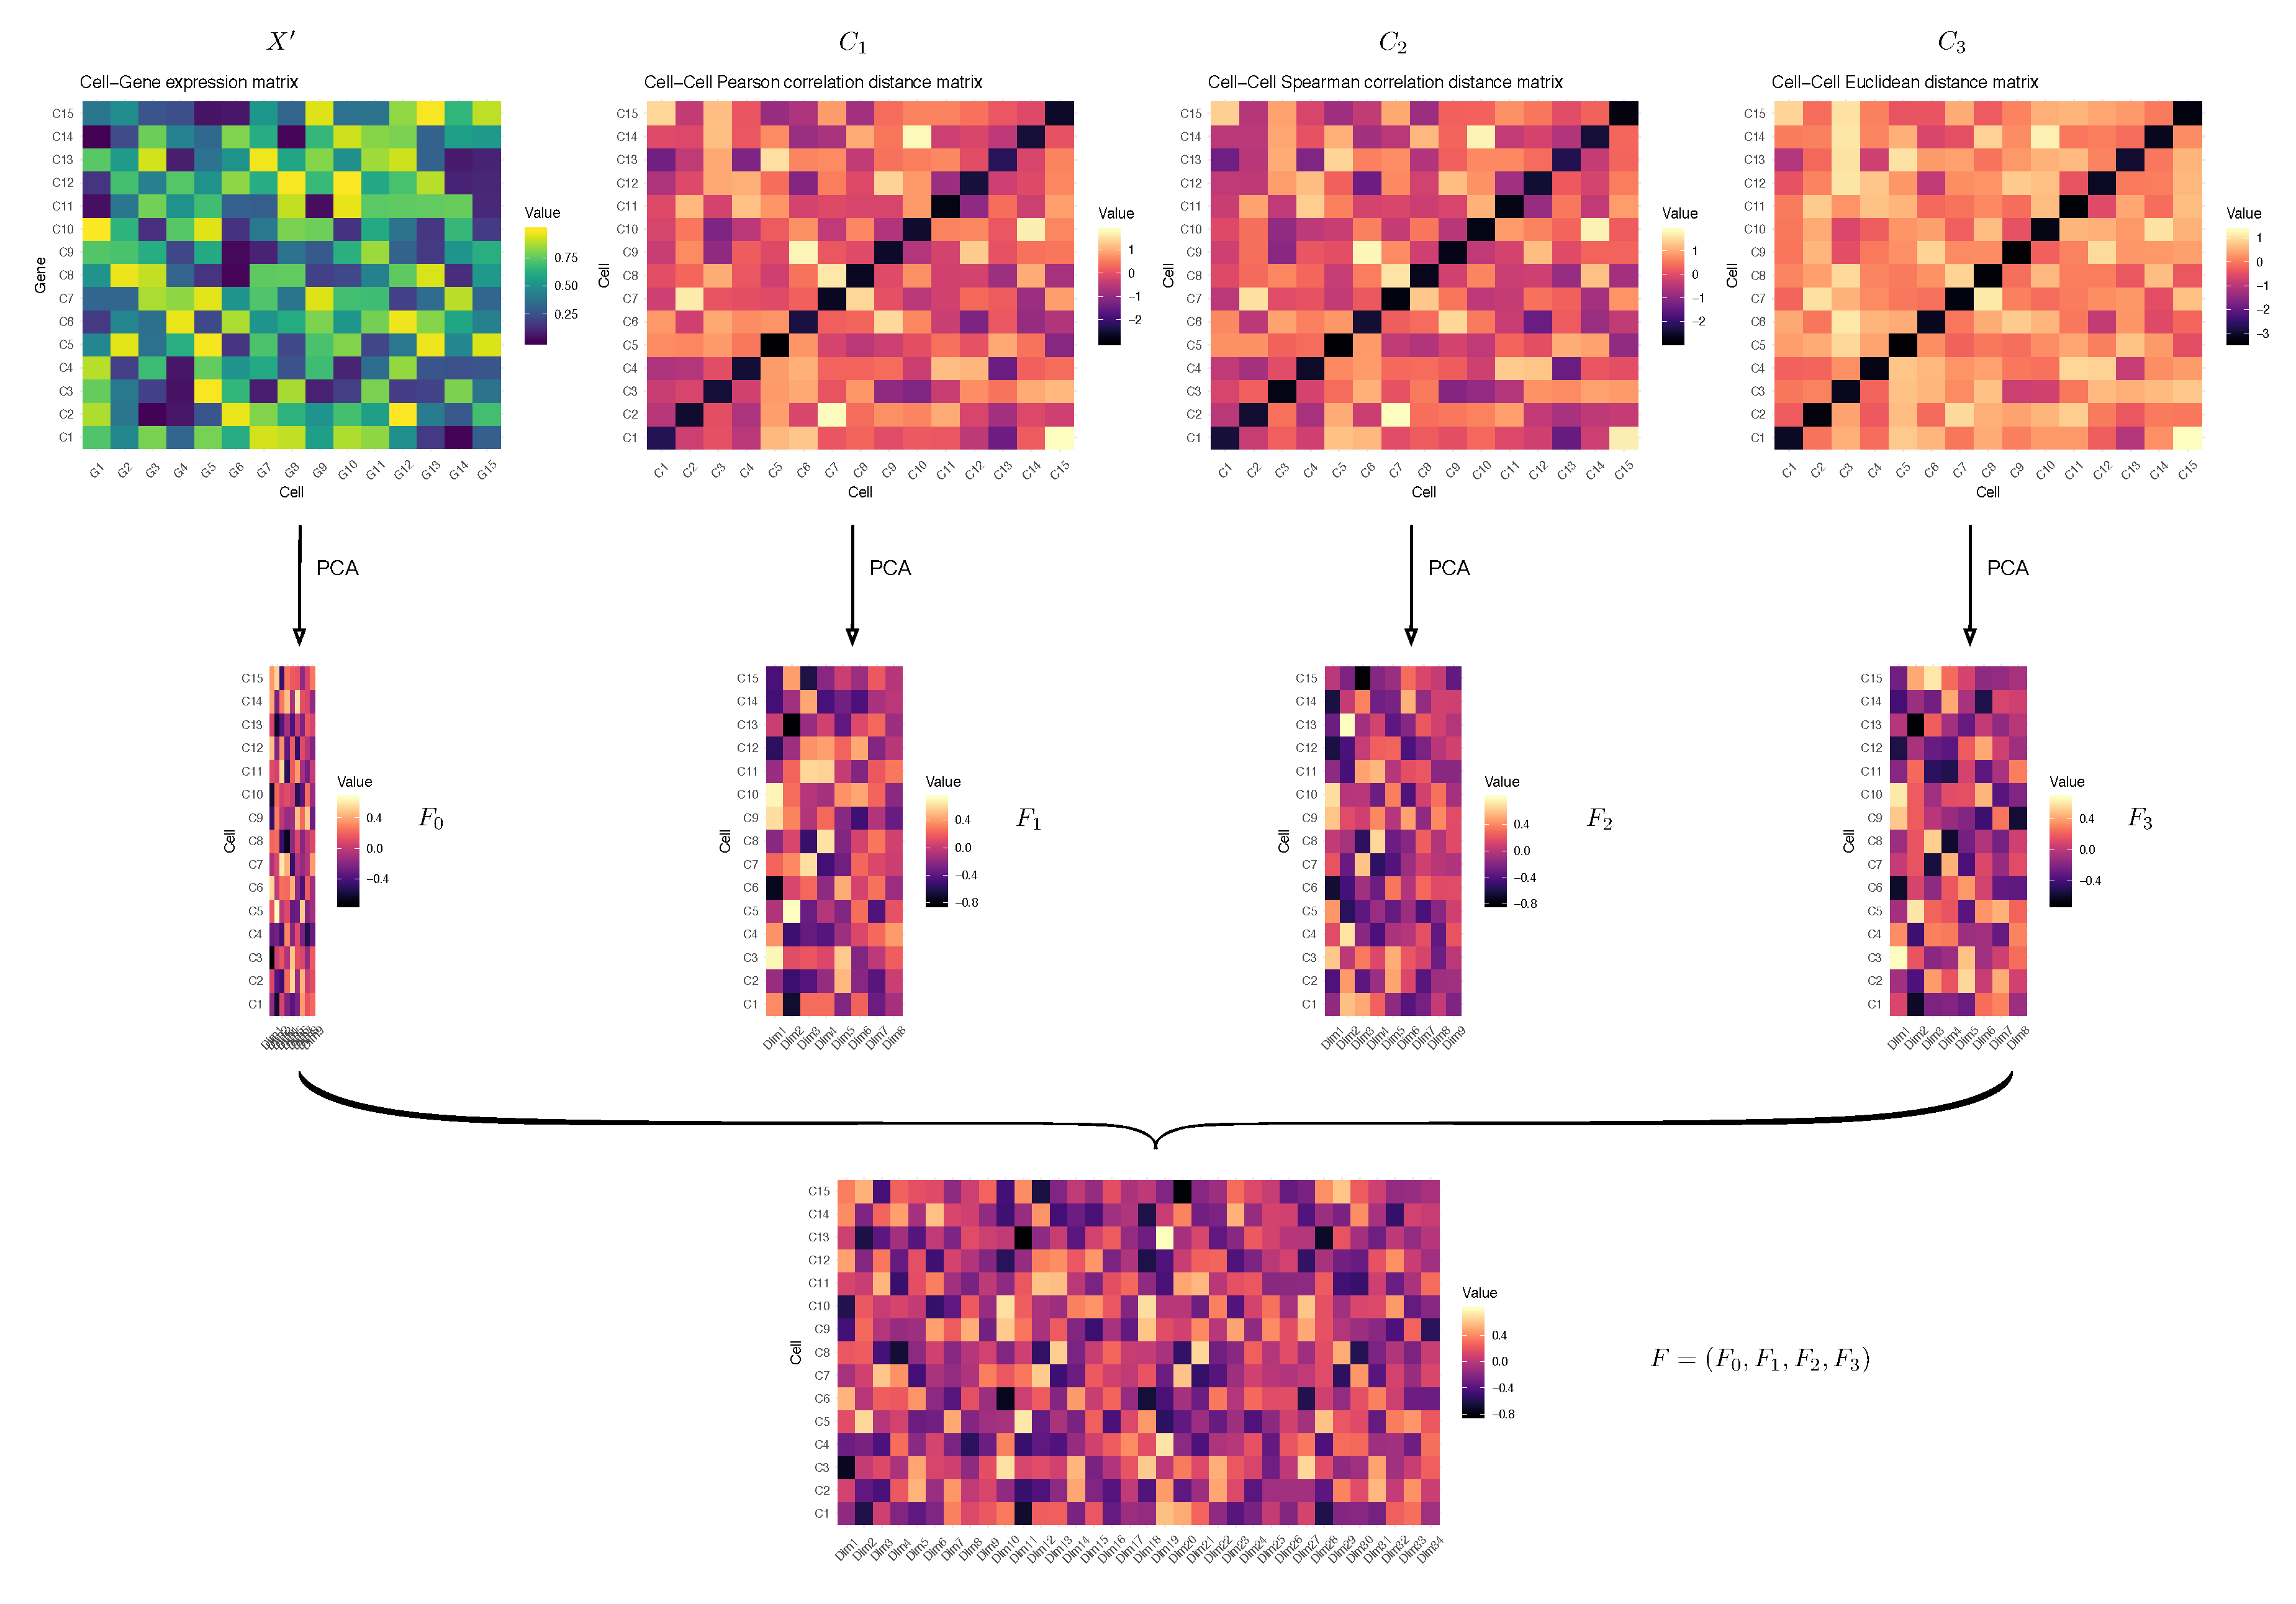
\includegraphics[width=0.9\textwidth]{rafsim.pdf}
    \caption{Illustration of the hand-crafted feature matrix construction in a toy dataset with 15 cells and 15 genes. The final feature matrix $F$ is in a $15 \times 34$ shape in this case}
    \label{fig:rafsim}
\end{figure}

RF~(随机森林,Random Forest)~是一种应用非常广泛的基于决策树的分类和回归方法~\cite{breiman2001random}。
另外,它也可以用无监督的方式来推断对象之间的相似性~\cite{shi2006unsupervised,breiman2011manual,pouyan2018random}。
另外,基于~RF~的相似性学习很容易适应于并行计算,
对离群值的鲁棒性,内在具有特征选择的特性,这些特点特别适合用来分析高维和噪声数据,
特别是像单细胞~RNA~测序图谱。
我们按照以下步骤来学习细胞-细胞的相似性。
在选择一个单一的特征~$j$~(特征矩阵~$F$~中的第~$j$~列)~后, 
我们使用围绕质心点的分区,并估计类别的数量,如由 
R包中的~\textit{pamk}~函数~\textit{fpc}~\cite{package-fpc}来获取该特征~$j$~的向量中的类标签。
然后,我们从~$F$~中去掉第~$j$~列,并且使用~RF~分类器对缩减后的数据集~$F_{-j}$~进行类别的标签学习。
让~$f_p$~表示~$F_{-j}$~的第~$p$~行,
如果~RF~分类器包含~$N$~树,并定义~$nt(f_p,f_q)$, 作为通过同一片叶子对细胞~$f_p$~和~$f_q$~进行分类的树的数量。
基于~RF~的~$n \times n$相似度矩阵~$S_j$是通过以下方式定义:
$S_{j_{pq}} = nt(f_p,f_q) / N, 1 \le p,q \le n$。
我们使用~R包\cite{package-randomforest},其默认森林大小为~500~棵,即~$N=500$。
对所有的~$\tilde{p}$~特征重复这个过程,得到~$\tilde{p}$~相似度矩阵~$S_j$,$j=1,2,\ldots,\tilde{p}$。
通过对所有~$S_j$~进行平均,得到最终的细胞-细胞相似度矩阵~$S$,
并通过~$D=1-S$~得到异质矩阵~$D$。

接下来,对异质矩阵~$D$,使用平均联结分层聚类来对细胞进行分组。
要对树枝图进行切割,可以使用~\textit{cutreeDynamic}~函数。
是使用了来自~\textit{dynamicTreeCut}的~R~包~\cite{langfelder2007defining,package-dynamicTreeCut}自动确定细胞的类别,
并为每个细胞分配正确的类标签。
另外,我们还提供了使用\textit{dynamicTreeCut}~R~包中的~\textit{cutree}函数来支持用户自定义细胞的类别数。


RafClust~旨在围绕细胞的类型或子类型的发现或表征。
在本研究中,应用~DoRC~的一个子程序~RafClust~来解决稀有细胞的异质性。
但实际上,它可以适应一般的单细胞聚类问题。
它是一种纯粹的无模型和数据驱动的方法,不需要其他的先验信息,如细胞或基因的群体结构、通路信息。
实验表明,RafClust~与其它知名的单细胞聚类方法相比具有一定的优越性。

RafClust~R包可在~\url{https://github.com/chenxofhit/RafClust}~免费下载和使用。

\subsubsection{差异基因分析}
\label{subsec:de}
在至少~2~个细胞中表达数超过~3~的基因被考虑进行后续分析。
我们使用~NODES~\cite{Sengupta049734}~这一快速的非参数化、差异化表达~(DE)~分析工具进行~DE~基因分析。
以~0.05~作为假发现率~(FDR)~的阈值,阈值的倍数变化为~log2(5)。
在~DE~基因中,在特定类中相对于其余各类显著上调的基因被命名为细胞类型特异基因。

\subsubsection{调整后的~Rand~指数和~F1得分}
聚类的效果是使用真实的类别标签~$L_T$和估计的类别标签~$L_E$之间的相似性来衡量,
使用的是调整后的~Rand~指数~\cite{hubert1985comparing,wu2005dynamic}:
\begin{equation}
\label{eq:ARI}
\resizebox{0.4\textwidth}{!}{$
    ARI(L_E,L_T)=\frac{\sum_{}{}_{e,t} \begin{pmatrix}n_{et}\\ 2\end{pmatrix} - \begin{bmatrix}  \sum_{}{}_{e} \begin{pmatrix}n_{e}\\ 2\end{pmatrix}\sum_{}{}_{t} \begin{pmatrix}n_{t}\\ 2\end{pmatrix}  \end{bmatrix} / \begin{pmatrix}n\\ 2\end{pmatrix} 
    }{\frac{1}{2}\begin{bmatrix}
    \sum{}{}_e\begin{pmatrix}n_{e}\\ 2\end{pmatrix} + \sum{}{}_t\begin{pmatrix}n_{t}\\ 2\end{pmatrix}
    \end{bmatrix} - \begin{bmatrix}
    \sum{}{}_e\begin{pmatrix}n_{e}\\ 2\end{pmatrix} \sum{}{}_t\begin{pmatrix}n_{t}\\ 2\end{pmatrix} 
    \end{bmatrix}/\begin{pmatrix}n\\ 2\end{pmatrix}}    
$}
\end{equation}
其中~$n$~是单细胞的总个数, 
$n_e$~和~$n_t$~分别是估计的类别~$e$~和真实的类别~$t$~中的单细胞数目; 
并且~$n_{et}$~是估计的类别~$e$~和真实的类别~$t$~共享的单细胞的数目。

ARI~的范围是~-1~到~1~,其中~1~表示估计的聚类与真实的聚类完全相同。
ARI~值越高,聚类算法的预测能力越强。

在两类实验中,直接构建一个混淆矩阵,其数字为真阳性~(TP)、假阳性~(FP)、真阴性~(TP)、假阴性~(FN)。
混淆矩阵上的精确性、召回率和~F1-score~可以很容易地计算如下:
\begin{equation}
    \label{eq:precision}
    \text{Precision} = \frac{\text{TP}}{\text{TP} + \text{FP}}
\end{equation}
\begin{equation}
    \label{eq:recall}
    \text{Recall} = \frac{\text{TP}}{\text{TP} + \text{FN}}
\end{equation}
\begin{equation}
\label{eq:f1score}
\text{F1-score} = 2 \times \frac{\text{Precision} \times \text{Recall}}{ \text{Precision} + \text{Recall}}
\end{equation}
在模拟实验中,对于其~DoRC~分数满足~IQR~阈值的标准的被认定为是稀有细胞。
对于实验中采用的~\textit{Jurkat\293T}~数据集,计算出~Jurkat~细胞的~F1~分数。


\subsection{实验结果}
\subsubsection{DoRC~概览}
\label{subsec:dorc}
RaceID~和~GiniClust~都依靠无监督聚类来检测稀有细胞。
RaceID~中的~\textit{k}-means~聚类是基于距离的,
而~GiniClust~中的~DBSCAN~聚类是基于密度的。
它们都属于基于近似的方法进行离群点检测。
基于近似的方法假设一个离群物体与其最近邻居的接近程度与该物体与数据集中大多数其他物体的接近程度有很大的差异。
聚类通常取决于一些敏感参数 且工作效率低下,因为不同分布的数据点之间的近似度不同。
另一个主要问题是决定群体身份的解析。
一般来说,多级聚类变得至关重要,因为次要的类经常在第一次筛选就被忽略~\cite{campbell2017molecular}。
发生这种情况是因为其他主要细胞类型会影响数据集中的表达差异,
特别是在处理大型~scRNA-seq~数据集时,情况变得更加糟糕。

为了解决上述问题,我们提出了发现稀有细胞~(DoRC),
这是一种从超大规模~scRNA-seq~数据中检测稀有细胞的非常快速的方法。
DoRC~的设计灵感来自于稀有细胞往往是``少而不同”的观察, 其中容易受到一种叫做孤立的机制影响。
孤立森林可以充分捕捉稀有细胞的特征,
其中,每个细胞的稀有性是以树枝的聚合长度为特征的。
一个细胞的长度越长,该细胞与其他细胞区分的因素就越多,它成为稀有细胞的可能性就越大。
从数量上看,孤立森林中的聚合异常分数具有本质上的稀有特征。
这为我们提供了自由度来调查和进一步决定细胞的稀有性。
为了说明这一点,我们将~DoRC~应用于包含~${\sim}68$k~外周血单核细胞的~scRNA-seq数据集~(PBMCs)~的注释进行比对,
这个数据集是知名的纯化的免疫细胞亚型数据集~\cite{zheng2017massively}。
他们首先对细胞进行了无监督聚类,
然后根据之前已知的标记对类进行注释~(图~\ref{supp-fig:dorcsummary} A)。
我们将~DoRC~的分数叠加在这一个小范围研究的二维图上~(图~\ref{supp-fig:dorcsummary} B)。
最高~0.1\%~的~DoRC~分数对应的是最小的, 
清楚地注释了含有巨核细胞的~CD34+~类别~(图~\ref{fig:dorcsummary} A)。
据报道,巨核细胞只含有整个剖析细胞的~0.3\%~\cite{zheng2017massively}。
然后,我们将这一比例从~0.1\%~增加到~1.0\%,随后又增加到~3.0\%,
下一批次的细胞亚型被选入扩展的稀有细胞集合中。
这些细胞包括单核细胞和树突状细胞亚型的亚类~(图~\ref{fig:dorcsummary} B-C)。
这个案例研究展示了~DoRC~在检测不同比例的稀有细胞方面的表现。

\begin{figure*}[!htbp]
    \centering
    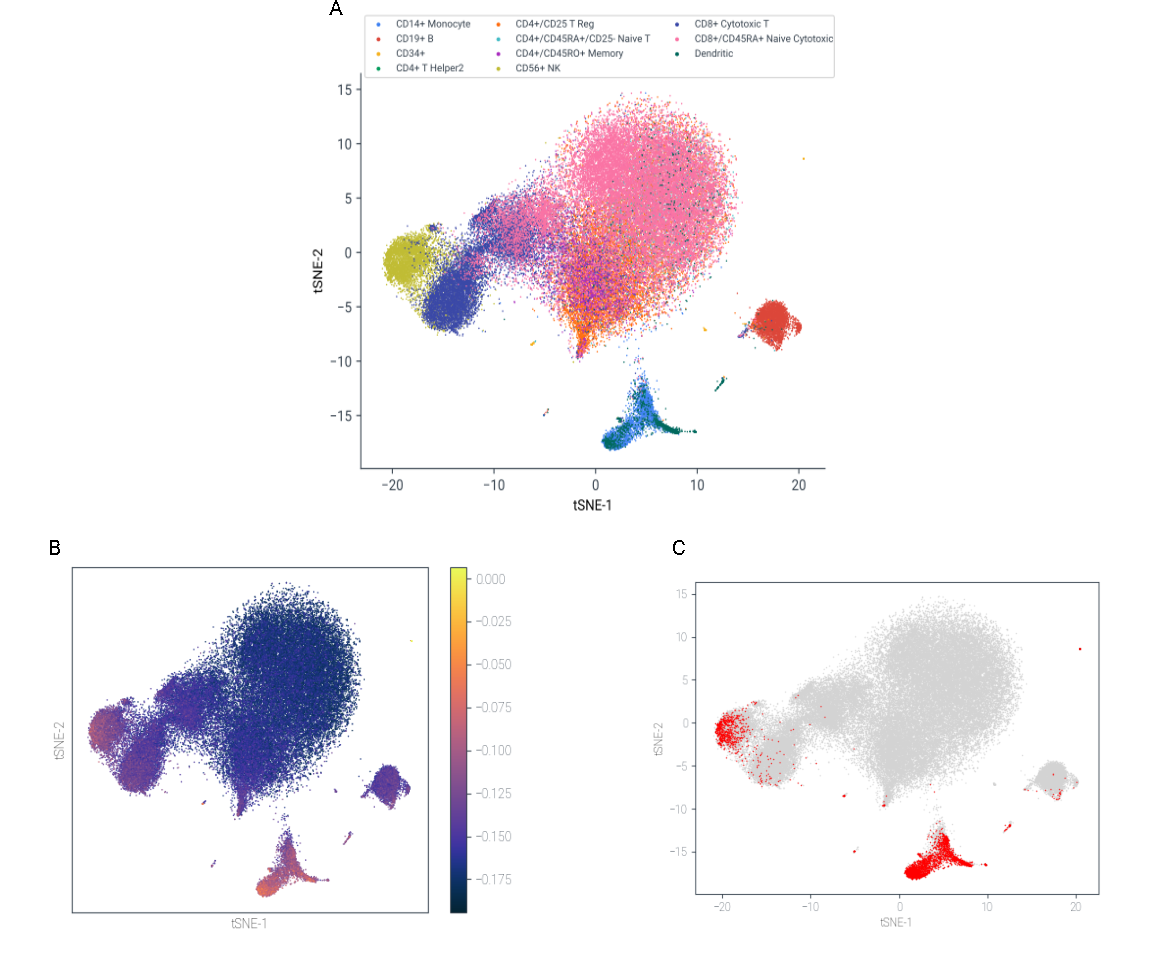
\includegraphics[width=0.9\textwidth]{DoRCSummarySI.pdf}
    \caption{Performance evaluation of DoRC on PBMCs\_68k. 
    (A) t-SNE based 2D embedding of the data with color-marked cluster identities as reported by Zheng et al.~\cite{zheng2017massively}. 
    (B) Heat map of DoRC scores for the cells on PBMCs\_68k. 
    The cluster of megakaryocytes (0.3\%), the rarest of all the cell types are assigned the
    highest DoRC scores.
    (C) Rare cells identified by DoRC using IQR-thresholding-criteria}
    \label{supp-fig:dorcsummary}
\end{figure*}

\begin{figure*}[!htbp]
    \centering
    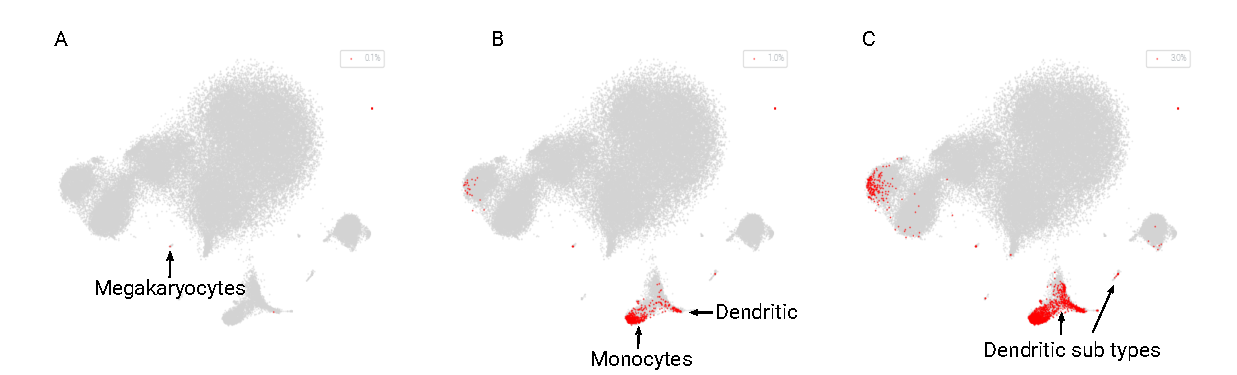
\includegraphics[width=0.9\textwidth]{DoRCSummary.pdf}
    \caption{DoRC discovers cells with varying degrees of rarity. In the ${\sim}68$k PBMC data~\cite{zheng2017massively}, minor cell populations with different grades of rarity show up with an
    increase in the number of selected rare cells. (A-C) The top 0.1, 1.0 and 3.0\% cells, respectively, selected on the basis of DoRC scores are highlighted}
    \label{fig:dorcsummary}
\end{figure*}

虽然连续的分数是有意义的,
有时候细胞稀有性的二元标注有助于后续的简化分析。
为了解决这个问题,我们引入了一个基于分数分布特性的阈值方法。
\ref{supp-fig:dorcsummary} C突出了~${\sim}68$k~PBMC~数据中检测到的细胞。
作为稀有细胞的基于阈值的二分法,
正如预期的那样,
大部分检测到的稀有细胞来源于已知的次要细胞类型,包括巨核细胞、树状细胞和单核细胞,
即分别是~CD34+、树枝状和~CD14+~单核细胞在~\ref{supp-fig:dorcsummary} A。

\subsubsection{RafClust~提高了~scRNA-seq~数据的聚类效果}

在本文提出的~RafClust~是为了区分稀有细胞的不同种类。
实际上,该方法对于任何一般的单细胞聚类都是可行的。
因此,为了验证~RafClust~在更一般情况下的性能,
我们将其应用在十个知名的~scRNA-seq~数据集上,这些~scRNA-seq~数据集从小规模到中等规模不等。
每个数据集以第一作者的姓氏命名如下: 
~\textit{Biase}~\cite{biase2014cell},
\textit{Treutlein}~\cite{treutlein2014reconstructing}, \textit{Pollen}~\cite{pollen2014low}, 
\textit{Kolod}~\cite{kolodziejczyk2015single}, \textit{Usoskin}~\cite{usoskin2015unbiased}, 
\textit{Zeisel}~\cite{zeisel2015cell}, \textit{Darmanis}~\cite{darmanis2015survey}, 
\textit{Tasic}~\cite{tasic2016adult}, 
\textit{Goolam}~\cite{goolam2016heterogeneity}, 
\textit{Li}~\cite{li2017reference}~(\ref{supp-tbl:clusteringdatasets})。
我们还将其结果~ARI~与其他六种基准方法进行比较,
包括~RaceID2~\cite{grun2016novo}, CIDR~\cite{lin2017cidr}, SIMLR~\cite{wang2018simlr}, SAFE~\cite{yang2018safe}, RtsneKmeans~\cite{hartigan1979algorithm,maaten2008visualizing,van2014accelerating}, RAFSIL~\cite{pouyan2018random}。
这六种聚类方法均以~R~包的形式实现并公开了代码,其概述见表~\ref{supp-tbl:clustereringmethods}~所示。
通过将每种方法的聚类结果与每个基准数据集的细胞类型注释进行比较,计算出对应的~ARI~值。 
实验在每个数据集上对每个方法重复~5~次,结果中位数的~ARI~值如图~\ref{fig:rafari}~所示,
由图~\ref{fig:rafari}~可知,RafClust~在~ARI~上优于其他六种方法。
我们还记录了每个方法在每个数据集上的执行时间,并将平均执行时间与其他基准方法进行比较,结果如图~\ref{supp-fig:clusteringtime}~所示。
由图~\ref{supp-fig:clusteringtime}~可知,RafClust~针对数据规模从小型到中型的~scRNA-seq~数据在计算效率上是可以接受的。

\begin{figure}[!htbp]
    \centering
    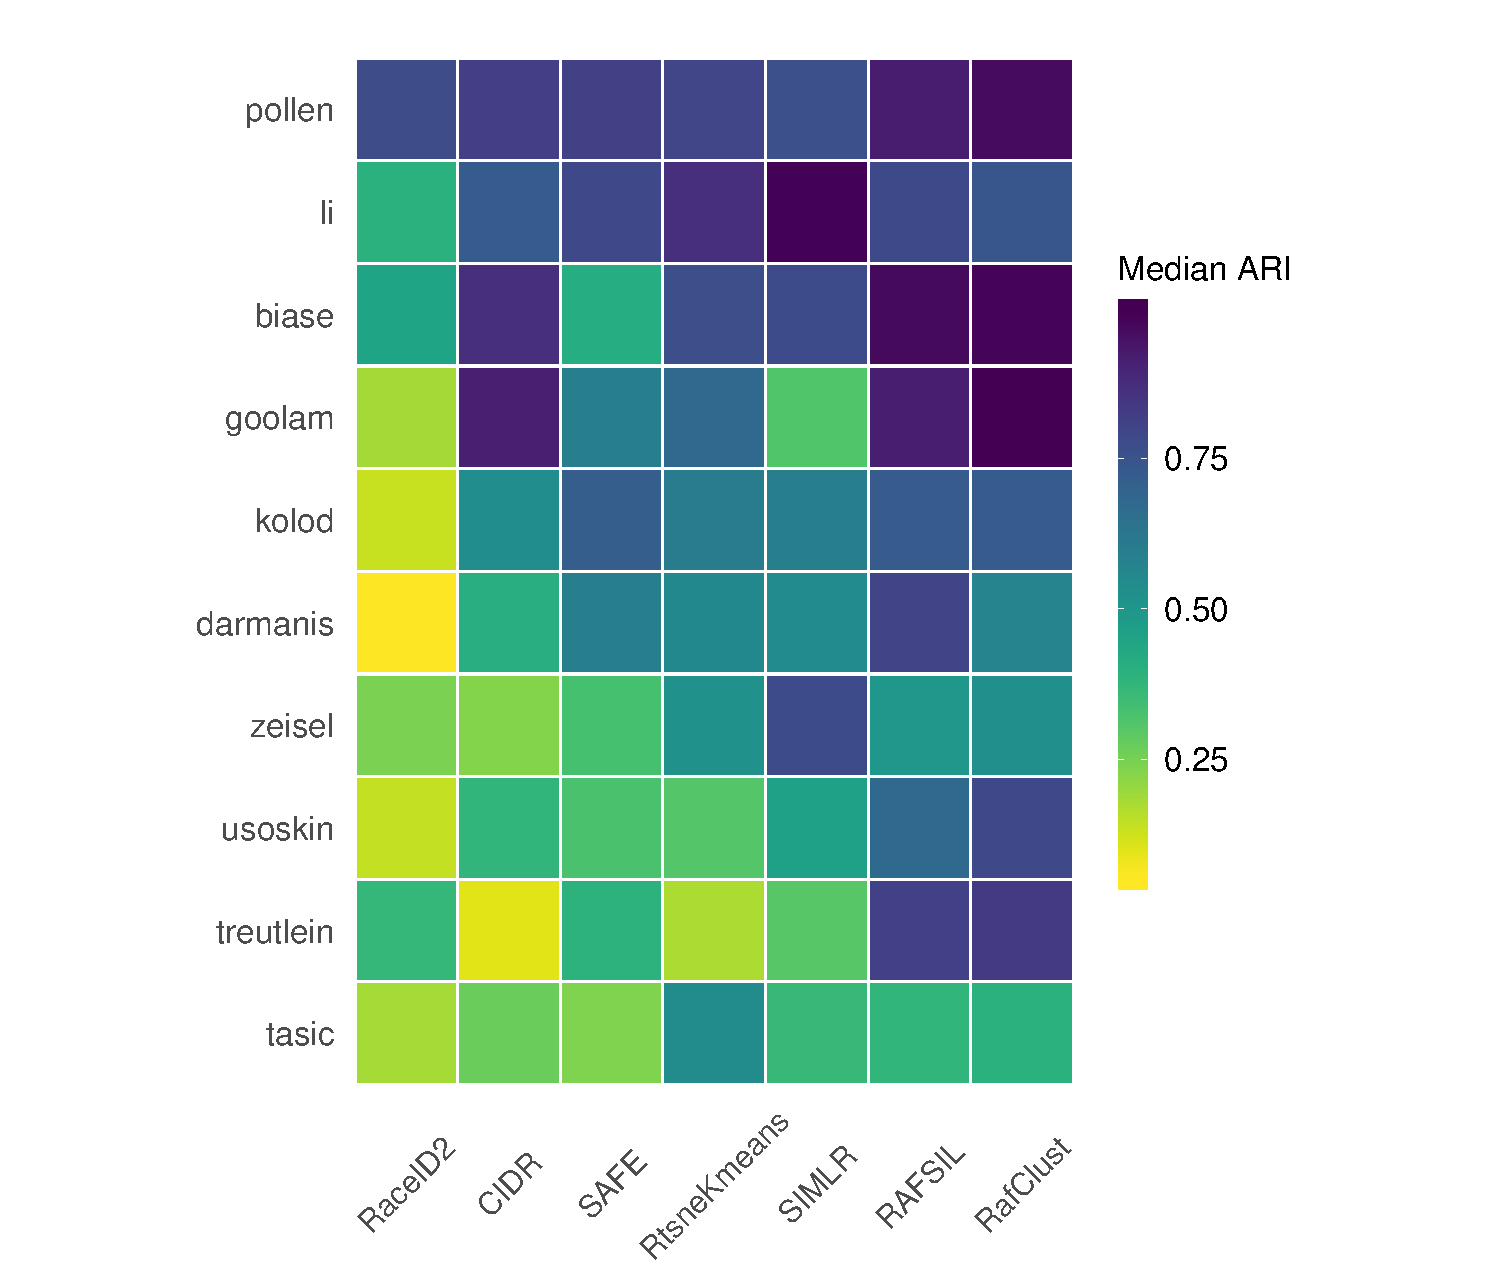
\includegraphics[width=0.9\textwidth]{Figure_ari_summary.pdf}
    \caption{Median ARI across different runs on the same dataset for the methods}
    \label{fig:rafari}
\end{figure}


\begin{table}[!htbp]
    \centering
    \caption{Overview of the  benchmark  datasets for the clustering performance comparison of RafClust with the other competing methods}
    \label{supp-tbl:clusteringdatasets}
    \resizebox{\columnwidth}{!}{%
    \begin{tabular}{llllrrrc}
    \toprule
    Dataset   &Accession 	&Sequencing protocol &Units &\#Cells &\#Genes	&\#Populations  & References \\
    \midrule
    Biase     &GSE57249     &SMARTer    &FPKM   &56	     &25 734     &5         &\cite{biase2014cell}\\
    Treutlein &GSE52583  	&SMARTer   	&FPKM  	&80      &23 271     &5 		&\cite{treutlein2014reconstructing}\\
    Pollen    &SRP041736 	&SMARTer   	&TPM   	&301     &23 730     &11 		&\cite{pollen2014low} \\
    %Patel     &GSE57872     &Smart-Seq 	&TPM   	&430     &5 948      &5			&\cite{patel2014single}\\
    Kolod     &E-MTAB-2600  &SMARTer    &CPM    &704     &38 616     &3         &\cite{kolodziejczyk2015single}\\
    Usoskin   &GSE59739  	&STRT-Seq  	&RPM   	&622     &25 334     &11 		&\cite{usoskin2015unbiased}\\
    Zeisel    &GSE60361     &STRT-Seq  	&UMI   	&3 005   &19 972     &9			&\cite{zeisel2015cell}\\
    Darmanis  &GSE67835  	&SMARTer    &CPM    &466     &22 088     &9         &\cite{darmanis2015survey}\\
    Tasic     &GSE71585     &SMARTer    &RPKM   &1 679   &24 057     &18        &\cite{tasic2016adult}\\
    Goolam    &E-MTAB-3321  &Smart-Seq2	&CPM  	&124     &41 480     &5			&\cite{goolam2016heterogeneity}\\
    Li     	  &GSE81861  	&SMARTer    &CPM   &561     &55 186      &9         &\cite{li2017reference}\\
    \bottomrule                   
    \end{tabular}
    }
    \begin{tablenotes}
        \small
        \item Note: These ten publicly available datasets are used as the benchmark datasets in this study.
        Seven of them are from~GEO (https://www.ncbi.nlm.nih.gov/geo/):\\~GSE57249,~GSE52583,~GSE59739,~GSE67835,~GSE71585,~GSE81861;
        ~two of them are from~ArrayExpress (https://www.ebi.ac.uk/arrayexpress/):~E-MTAB-2600,~E-MTAB-3321; 
        and the last one is from SRA~(Sequence Read Archive,\\~https://www.ncbi.nlm.nih.gov/sra):~SRP041736. 
        Each dataset is named as the first author's surname. 
        If two or more files are available in different units, 
        we only download the file in the corresponding unit shown in the ``Units" column.
        The numbers of cells, genes, and populations delivered in each dataset are also summarized in this table.
        These ten datasets are also available in \url{https://hemberg-lab.github.io/scRNA.seq.datasets}, 
        which contains a collection of publicly available datasets in this field.
      \end{tablenotes}
    \end{table}

\begin{table}[!htbp]
        \centering
        \caption{Overview of the benchmark clustering methods}
        \label{supp-tbl:clustereringmethods}
        \resizebox{\columnwidth}{!}{%
            \begin{tabular}{lll}
            \toprule
            Method                                                                     & Description                                                                                                                                                        & Reference \\
            \midrule
            CIDR (v0.1.5)                                                              & PCA dimension reduction based on zero-imputed similarities, followed by hierarchical clustering                                                                    & \cite{lin2017cidr}         \\
            \begin{tabular}[c]{@{}l@{}}RaceID2 (March 3, \\ 2017 version)\end{tabular} & K-medoids clustering based on Pearson correlation dissimilarities                                                                                                  & \cite{grun2016novo}        \\
            RtsneKmeans                                                                & \begin{tabular}[c]{@{}l@{}}t-SNE dimension reduction (initial PCA dim=50, t-SNE dim=3, perplexity=30) and K-means \\ clustering with 25 random starts\end{tabular} & \cite{hartigan1979algorithm, maaten2008visualizing,van2014accelerating}        \\
            SAFE (v2.1.0)                                                              & Ensemble clustering using SC3, CIDR, Seurat and t-SNE + Kmeans                                                                                                     & \cite{yang2018safe}         \\
            SIMLR                                                                      & An appropriate cell to cell distance metric by multi-kernel learning, followed by spectral clustering                                                                                                                                                          & \cite{wang2018simlr}         \\
            RAFSIL                                                                     & Random forest based cell to cell similary learning, followed by Kmeans or hierarchical clustering                                                                                                                                                              & \cite{pouyan2018random}        \\
            \bottomrule
        \end{tabular}
        }
    \end{table}
    
    \begin{figure}[!htbp]
        \centering
        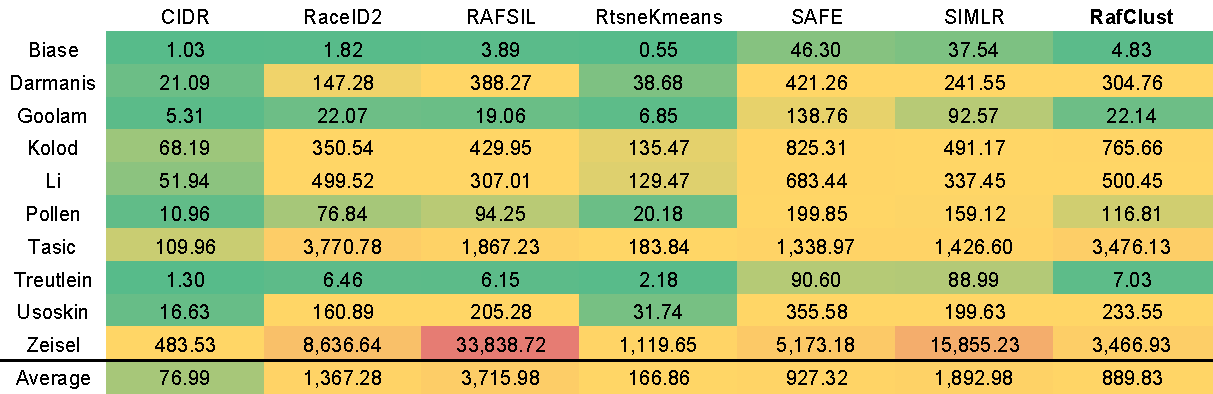
\includegraphics[width=0.9\textwidth]{Exp_RafClust_time.pdf}
        \caption{Median execution time details (in seconds) across  different runs for each dataset with the benchmark methods. 
        The time measurements were taken on a workstation that running GNU Linux/Ubuntu 16.04 operating system with 4.15.0-46-generic kernel with the
        following hardware configuration: Intel(R) Xeon(R) CPU E5-2630 v4 @ 2.20GHz with 40 cores and 256 GB of RAM.}
        \label{supp-fig:clusteringtime}
    \end{figure}

\subsubsection{DoRC揭示了树突状细胞之间的异质性}
树突状细胞~(DC)~在感知、吞噬和和抗原监视~\cite{villani2017single}~方面起着至关重要的作用。
DCs~是最罕见的免疫细胞类型之一,构成约~0.5\%~的~PBMCs~\cite{zheng2017massively}。
Villani~\cite{villani2017single}的研究划分了六种不同的树突状细胞的亚型。
通过荧光激活细胞分选~(FACS)~分析树突状细胞的表达,分选的~DCs~和单核细胞的情况图。
他们在研究中报告的~DC~亚型如下:
$\text{CD141}^+$ DCs (DC1), 
$\text{CD1C}^+${\_}A 常规 DCs (DC2),
$\text{CD1C}^+${\_}B 常规 DCs (DC3),
$\text{CD1C}^-\text{CD141}^-$ (DC4), DC5~和浆细胞~DCs (DC6, pDCs)。

我们很好奇树突状细胞亚型是否可以在~PBMCs~数据中被识别。
首先,我们在~${\sim}68$k PBMCs~数据集上应用~DoRC。
DoRC~通过使用基于~IQR~的二分法,共发现了~3844~个稀有细胞。
然后通过~RafClust~对稀有细胞进行聚类~(见~\ref{subsec:rafclust}),得到~12~个子类别。
在这~12~个可区分的聚类中~(C0-C11),
C4、C5、C9~和~C11~完全由树枝状细胞组成,根据~Zheng~等人提供~\cite{zheng2017massively}的注释,
如图~\ref{fig:dorc_dendritic} A-C~所示。
对于这~4~个~DC~类别,我们进行差异表达分析,找出细胞类型特异性基因~(见~\ref{subsec:de})。
共有~21~个基因被检测为细胞类型特异性基因,使用截止~log2(1.5)~的~FC~(fold change)。
通过将我们的差异基因与~Villani~\cite{villani2017single}~报道的基因进行叠加。
我们可以有信心地解析~6~个亚型中的~5~个~(DC1、DC2、DC4、DC6)~(图~\ref{fig:dorc_dendritic} D、表~\ref{supp-tbl:dendritic})。
从~\cite{villani2017single}~可以看出,DC5~是未解决的,因为该类型是新分离的罕见类型。
在基于~t~分布的随机邻域嵌入~(t-SNE)~的二维嵌入图中,DC3~与~DC2~属于同一类~\cite{maaten2008visualizing}。
在~DoRC~检测到的稀有细胞上进行~RafClust~聚类,不能完全划分出树突状细胞亚型正确的数量。
然而,在最初~\cite{zheng2017massively}的研究中,DC1~和~DC4~并没有被无监督聚类解决。
事实上,在~t-SNE~图中~\cite{zheng2017massively},
这些细胞类型在视觉上共同聚集在自身或单核细胞内。
\begin{figure}[!htbp]
    \centering
    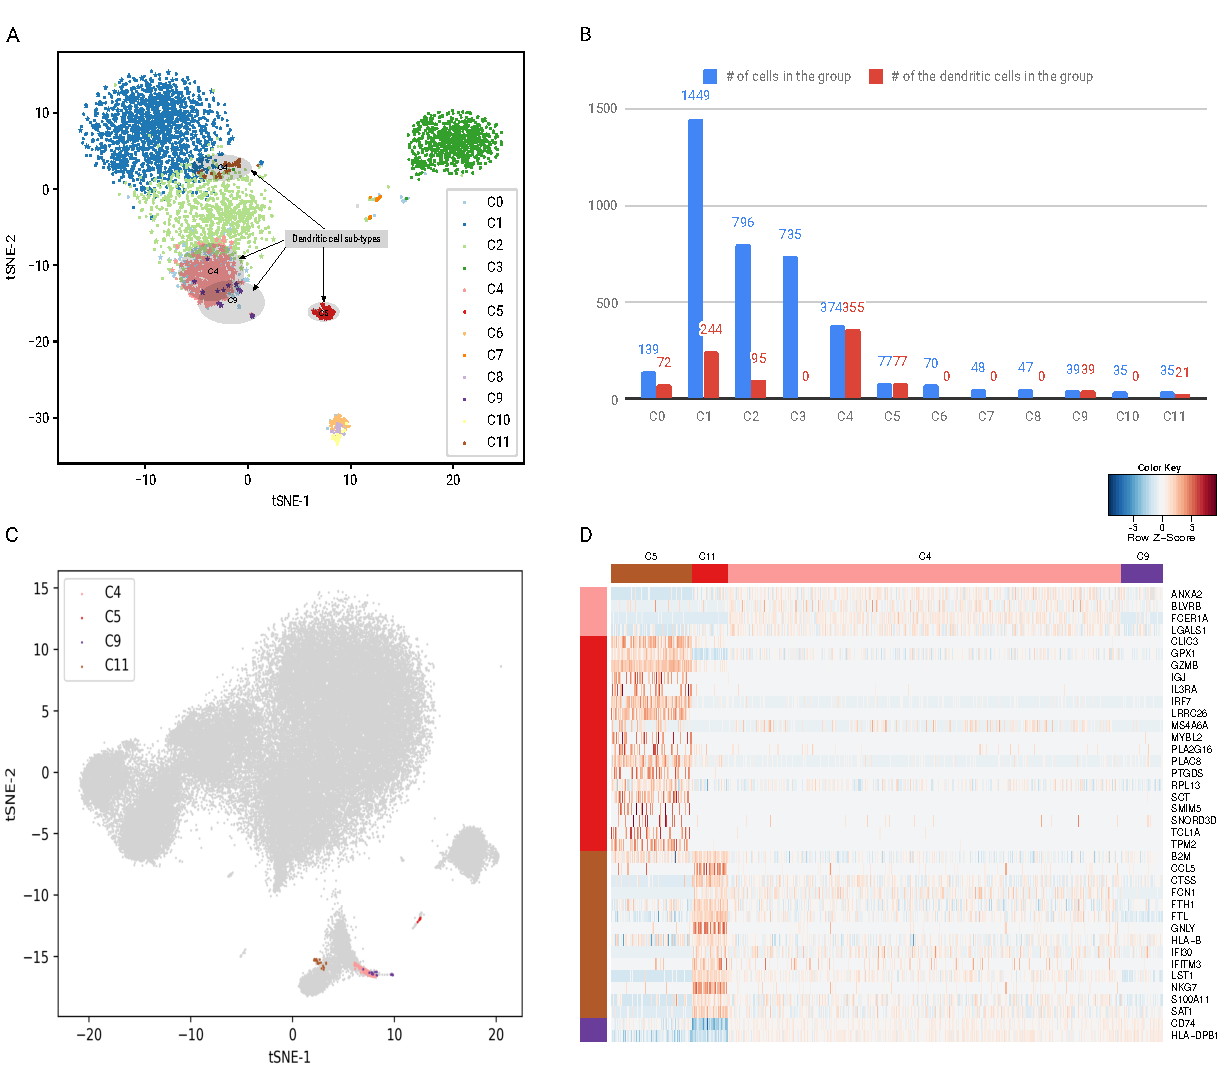
\includegraphics[width=0.9\textwidth]{plot_tsne_dorc_rare_summary.pdf}
    \caption{Human blood dendritic cell heterogeneity delineated by DoRC. 
    (A) DoRC detected rare cells are clustering into 12 sub types with RafClust, 
    i.e.~C0 (a singleton class), C1, $\ldots$, C11.
    With the annotation given by~\cite{zheng2017massively}, C4, C5, C9, C11 are mostly dendritic cells sub types.
    Dots with the same color represent one subpopulation by clustering the rare cells with RafClust.
    For each subpopulation, the cells annotated with asterisks marking are also dendrotic cells according to the annotation given by~\cite{zheng2017massively}. 
    (B) The cells number for each subpopulation and the number of dendrotic cells in this group. 
    Apparently, dendritic cells hold the majority of the subpopulation in C4, C5, C9, C11.
    (C) These four dendritic sub-types cells are highlighted on the~\textit{PBMCs\_68k} dataset t-SNE-based 2D plot.
    (D) Characterization of dendritic cell sub-types utilizing markers obtained from DE analysis (See~\ref{subsec:de})}
    \label{fig:dorc_dendritic}
\end{figure}

\begin{table}[htbp]
    \centering
    \caption{The dendritic cell types correspond to class types reported by Villani~\cite{villani2017single}}
    \label{supp-tbl:dendritic}
    \resizebox{\columnwidth}{!}{
    \begin{tabular}{|c|l|c|}
    \hline
    Class type & \multicolumn{1}{|c|}{Marker gene(s)}                                                                                                                                   & Corresponding class type \\ \hline
    C4         & ANXA2, BLVRB, \textbf{FCER1A}, LGALS1	                                                                                                                                         & DC2                      \\ \hline
    C5         & \begin{tabular}[c]{@{}l@{}}CLIC3, GPX1, \textbf{GZMB}, \textbf{IGJ}, \textbf{IL3RA}, \textbf{IRF7}, LRRC26, MS4A6A, MYBL2,\\ PLA2G16, PLAC8, PTGDS, RPL13, SCT, SMIM5, SNORD3D, TCL1A, TPM2\end{tabular} & DC6                      \\ \hline
    C9         & \begin{tabular}[c]{@{}l@{}}B2M, CCL5, CTSS, FCN1, FTH1, \textbf{FTL}, GNLY, HLA-B, IFI30, \textbf{IFITM3}, \textbf{LST1},\\ NKG7, S100A11, SAT1\end{tabular}                                    & DC4                      \\ \hline
    C11        & CD74, \textbf{HLA-DPB1}                                                                                                                                                       & DC1                      \\ \hline
    \end{tabular}
    }

    \begin{tablenotes}
        \small
        \item Note: Those genes marked in bold are  acting as  marker genes in the corresponding class type.
      \end{tablenotes}

\end{table}

\subsubsection{DoRC~能够识别人工伪造的稀有细胞}
\label{subsec:recplanted} 
我们设计了一个模拟实验来评估~DoRC~关于细胞类型识别相关的事实真实信息的性能。
我们使用了一个~scRNA-seq~数据集~Jurkat\_293T,由~293T~和~Jurkat~细胞在体外以不同比例混合组成~(见节~\ref{subsec:datasets})。
作者利用每个细胞的单核苷酸变异~(SNV)~谱来确定其系谱。
我们认为这种基于基因型的注释方案接近于事实。

随着~Jurkat~(稀有)~细胞在所有细胞中的占比变化,比例从~0.5\%~到~15\%,
我们得到八个数据集。
对于每个数据集,F1-score~是用通过~DoRC~评分和~IQR~阈值标准确定预测标签,然后与两个类的真实标签对照计算。
重复这个过程~100~次,可以得到该数据集的~F1~分数的标准差。
标准差反映了该方法识别人工伪造的稀有细胞的稳定性~(图~\ref{fig:jurkat} A)。 
F1-score~反映了精度和灵敏度之间的平衡。
当稀有比处于低水平时,即~0.5\%~和~1\%~时,DoRC~无法匹配~FiRE。
但是,当稀有率从~1.5\%~增加到~15\%~时~DoRC~的性能优于~FiRE。
此外,FiRE的性能在~15\%~的罕见比例下急剧下降,但是~DoRC~更保守,性能损失较小。

我们仔细研究一下在稀有细胞占比为~2.5\%~时的细节。
从~100~个生成的数据集中随机选取了一个有~1539~个细胞的混合数据集,作为基准数据集。
~39~个稀有细胞和~1500~个丰富细胞非常清晰地聚成两组~(图~\ref{fig:jurkat} B)。
在这两种方法中,稀有细胞的得分都毫不含糊地高于丰富细胞类型~(图~\ref{fig:jurkat} C-D)。
与每个方法得到的二元注释~(图~\ref{fig:jurkat} E-F),
DoRC的表现优于~FiRE,
因为它有更高的能力来检测更多的稀有细胞~(图~\ref{fig:jurkat} G-H)。

\begin{figure}[!htbp]
    \centering
    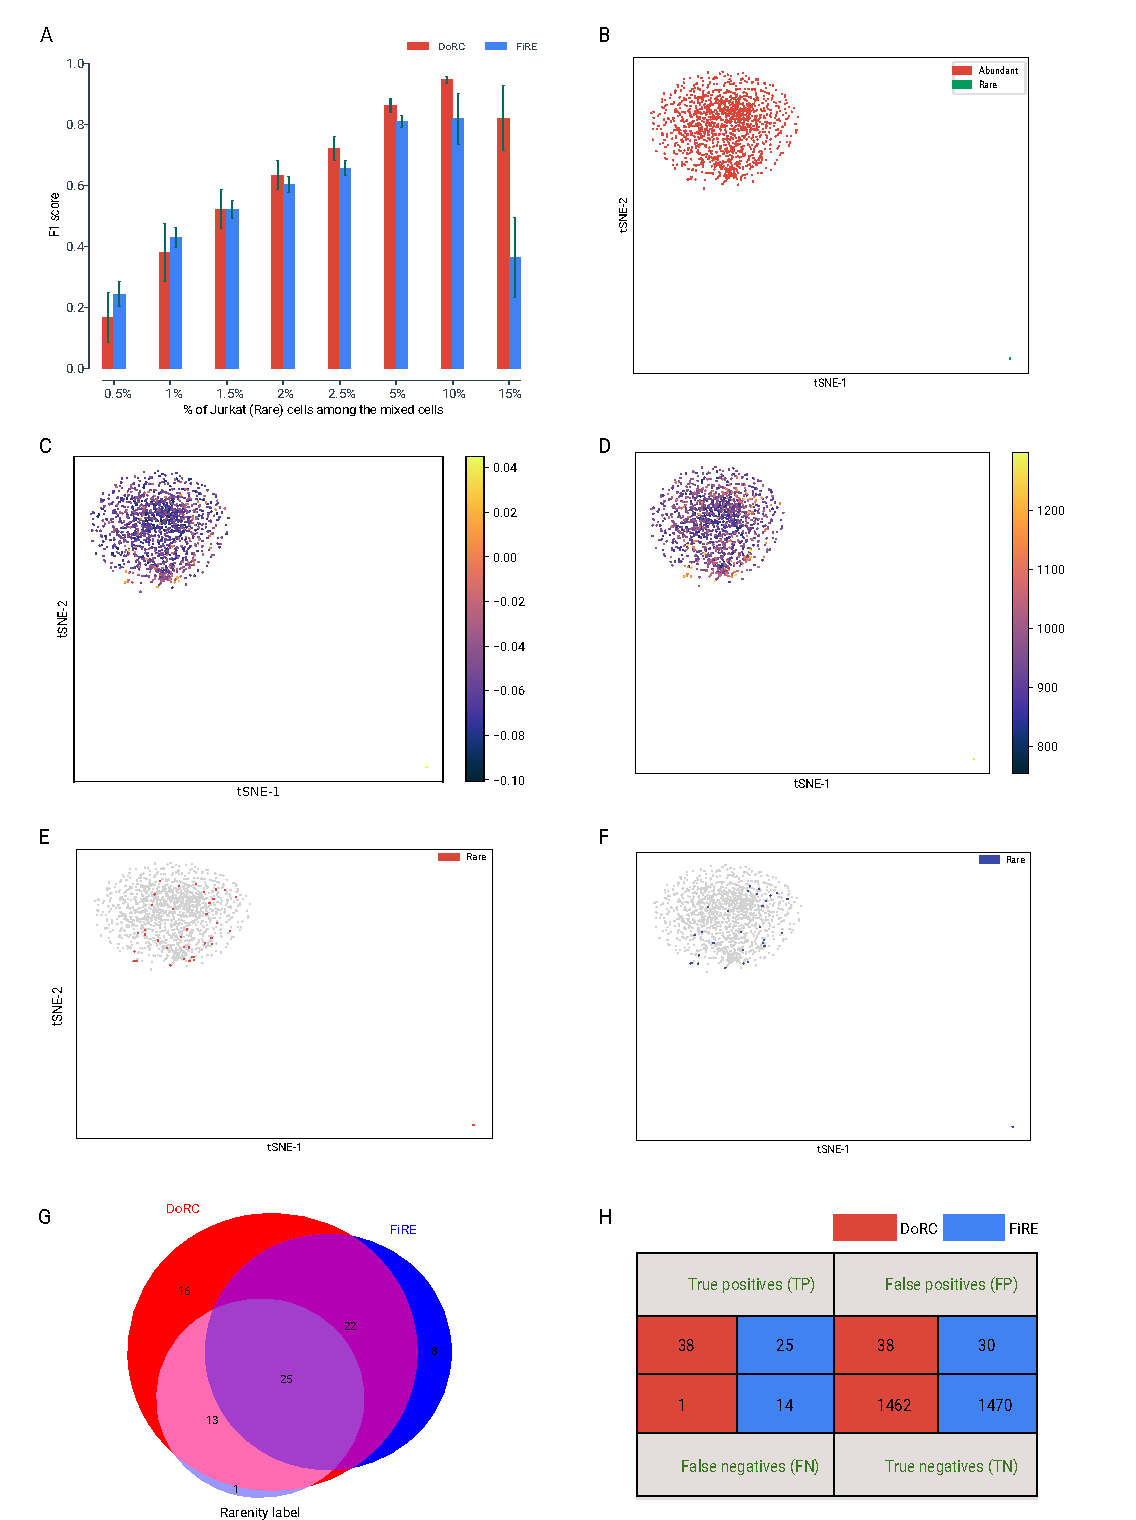
\includegraphics[width=0.9\textwidth]{plot_venn_dorcfire_39summary.pdf}
    \caption{Detectability of minor cell types in a simulated dataset consisting of Jurkat and 293T cells. 
    (A) The F1-scores are calculated w.r.t. the rare (Jurkat) population for DoRC and FiRE, 
    while bioinformatically varying the proportion of artificially planted rare cells.
    (B) The t-SNE-based 2D embedding of the cells with color-coded identities of the benchmark dataset.
    (C-D) DoRC and FiRE score intensities plotted on the t-SNE-based 2D map, respectively. 
    (E-F) The rare cells detected by DoRC and FiRE, respectively, are highlighted.
    (G) DoRC, FiRE detected rare cells and true rare cells overlap with each other, shown in this Venn diagram. 
    (H) Detail of the confusion matrices with TP, FP, FN, TN prediction metrics for DoRC and FiRE.}
    \label{fig:jurkat}
\end{figure}

\subsubsection{DoRC~对细胞类型敏感}
我们设计了一项模拟研究来分析~DoRC~评分的鲁棒性和敏感性与差异表达基因数量的关系。
我们首先生成一个由~500~个两种细胞类型组成的人工~scRNA-seq~数据。
数量小的细胞类型约占细胞的~5\%~(见节~\ref{subsec:datasets})~。
我们将通过严格的标准选择的差异表达~(DE)~基因保留在一边。
对于每次实验的迭代,我们将预先确定的~DE~基因附加到固定数量的非~DE~基因上。
我们在~1~和~150之间改变差异表达基因的计数,以跟踪~DoRC~在检测规模小的类别细胞的敏感性。
随着给定的~DE~基因集合,计算获得~DoRC~分数,并对小类别细胞进行计算受试者测试工作曲线~(ROC)~下面积~(AUC)~。
对于每一种数量的~DE~基因,上述过程重复~1000~次。
汇总后的平均~AUC,以及所有的~AUC~的标准差如图~\ref{fig:simulate:roc}~中所示。
随着~DE~基因数量的减少,DoRC~难以检测到次要细胞群。
然而,当引入~20~个或更多的~DE~基因时,DoRC~的预测率急剧提升。
同时,随着偏差变小,预测变得更加稳定。
另外从给出的~t-SNE~图来看,由于~DE~基因的增加,两类细胞能够更加直观地区分出来。
这个实验反应了~DoRC~对噪声的鲁棒性。

\begin{figure}[!htbp]
    \centering
    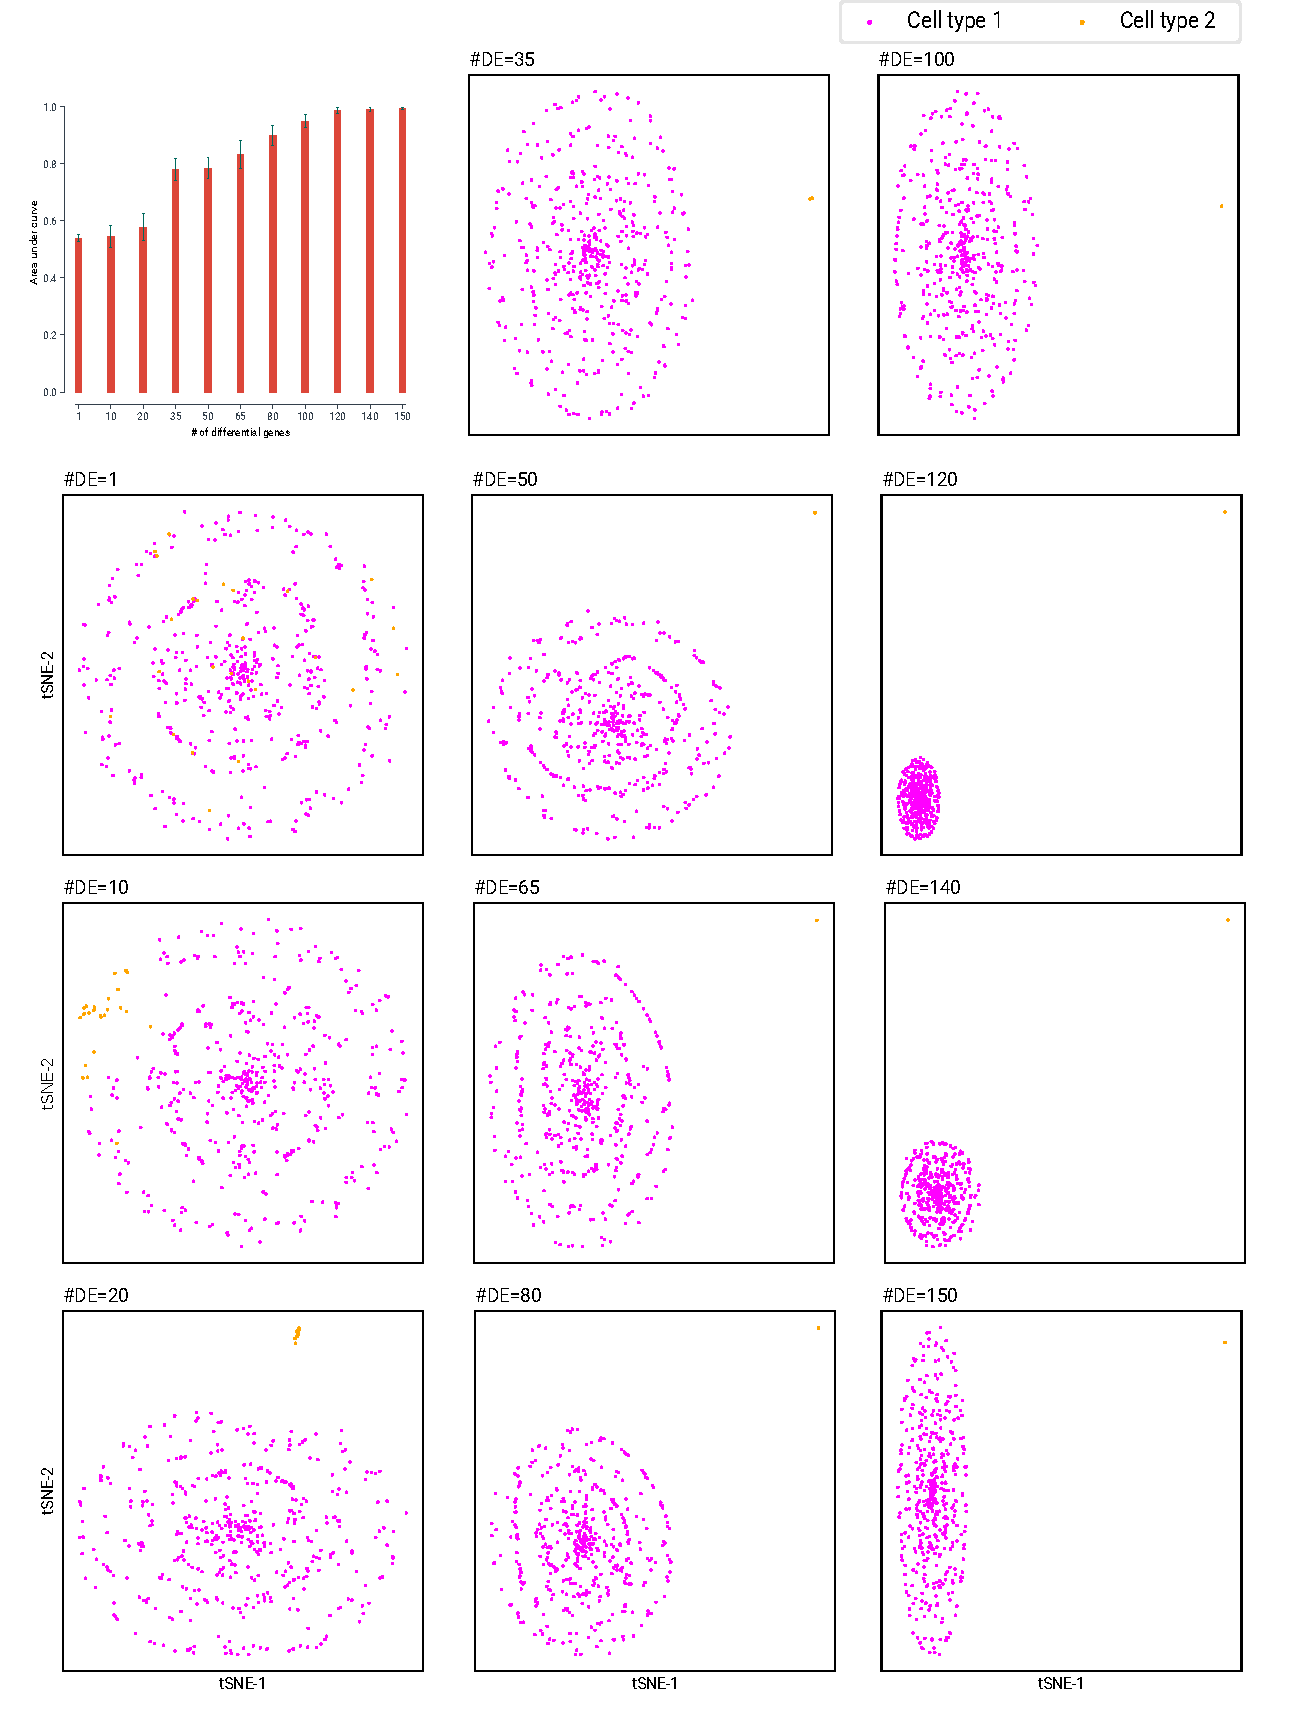
\includegraphics[width=0.9\textwidth]{simulate_panorama.pdf}
    \caption{The sensitivity of DoRC to cell-type identities. 
    On the scRNA-seq dataset \textit{Splatter\_500}, 
    DoRC starts with recognizing the minor cell type correctly, 
    as soon as the number of differentially expressed genes becomes adequate to give rise to a tiny cluster representing the minor cell
    subpopulation. 
    The top-left corner figure serves as a legend for the subsequent AUC plots. 
    Each t-SNE and ROC plot pair serves as a representative of the 1000 repetitions of the experiment concerning a
    specific number of differentially expressed genes. 
    The AUC analysis is performed using cell-type annotations, 
    and DoRC scores are assigned to individual cells.}
    \label{fig:simulate:roc}
\end{figure}

此外,由于~DoRC和~FiRE都可以给一个细胞做二元标注,
我们对其性能差异感到好奇。
在这个数据集中,我们考虑了~DoRC和~FiRE之间的~AUC、召回率、精度和~F1-score。
由于~F1-score~取决于召回率和精度,我们也包括这两个指标作为参考。
把细胞类型标注为真实标签,AUC~是用~DoRC~评分计算的。
而~F1-score是用~DoRC~评分产生的稀有度标注与~IQR~阈值标准获得的。
在总共~25~个稀有细胞中,DoRC~和~FiRE~都能正确检测出~23~个相同的稀有细胞。
DoRC~可以检测到其他~2~个稀有细胞和~1~个假阳性稀有细胞,
而~FiRE未能识别出左边~2~个稀有细胞~(图~\ref{fig:simulate:venn_auc_f1}A)~。
在这个数据集中, 阳性样品~(丰富细胞)~和阴性样品~(稀有细胞)~的数量是不平衡的。
这两种方法的~AUC~和精度基本没有变化,
但~DoRC的召回率和~F1-score均高于~FiRE (图~\ref{fig:simulate:venn_auc_f1}B)。
\begin{figure}[!htbp]
    \centering
    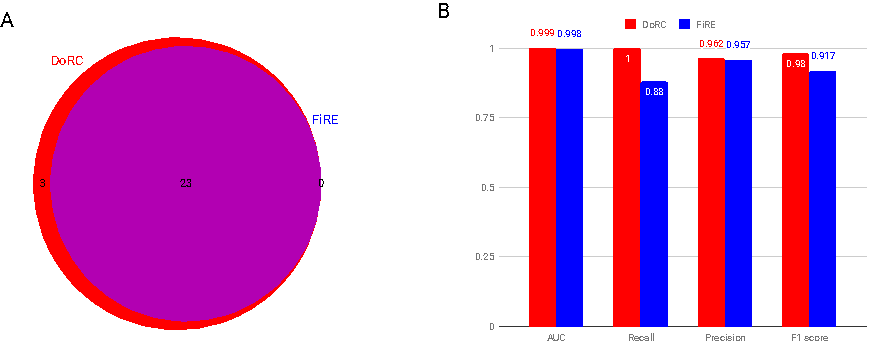
\includegraphics[width=0.9\textwidth]{plot_venn_dorcfire.pdf}
    \caption{Comparsion of DoRC and FiRE for rare cells detection in the dataset~\textit{Splatter\_500}.
    (A) Among all the 25 rare cells,  23 rare cells are all detected by DoRC and FiRE. 
    DoRC could detect other 2 rare cells and 1 false positive rare cells, 
    while FiRE failed to identify the left 2 rare cells.
    (B) The AUC and precision of DoRC and FiRE are almost the same, while the Recall and  F1-score of DoRC is higher than FiRE.}
    \label{fig:simulate:venn_auc_f1}
\end{figure}

\subsubsection{DoRC是可扩展和快速的}
\label{subsec:scalable} 
DoRC的核心算法孤立森林~(Isolation Forest)~的时间复杂度为~$O(ntlog\psi)$~\cite{liu2008isolation}。
其中~$n$、$t$~和~$\psi$~分别代表样本数、树的数目和每棵树的子样本数。
值得注意的是,DoRC~中的~Isolation Forest~在这种情况下没有训练的阶段。
该方法的参数我们使用默认值,~t~设置为~100,$\psi$~设置为~256。
因此,DoRC~的时间复杂度为~$O(n)$。
RafClust~的稀有细胞类型细化的复杂性没有考虑。
因为如果不需要稀有细胞的类型,这个步骤是可选的,FiRE~和~LOF~这两种方法中也没有包含这个步骤。

我们改变输入数据大小,
统计了~DoRC、FiRE、GiniClust、LOF~\cite{breunig2000lof}和~RaceID所花费的时间,
如图~\ref{fig:timecomplexity}所示。
测试机器为一台运行~GNU Linux/Ubuntu 16.04操作系统~4.15.0-47-generic~内核的工作站上,
硬件配置如下:Intel(R) Xeon(R) Silver 4116 CPU @ 2.10GHz,48~核,64GB~内存。
DoRC由~Python实现,使用scikit-learn包~(版本0.20.2)~~\cite{pedregosa2011scikit}和~pyod包~(版本0.6.7)~~\cite{zhao2019pyod}。
由于其他方法不能区分稀有细胞类型,在DoRC中我们也因此省略~RafClust的稀有细胞类型细化子程序。
FiRE从~\url{https://github.com/princethewinner/FiRE}下载(分支:master,最新提交的~abcba5b)。
因为其内核算法是用C++编写的,我们在实验中使用的是其~Python~扩展分支。
GiniClust从~\url{https://github.com/lanjiangboston/GiniClust}下载~(分支:master,最新提交~a442d45)。
我们在命令行界面直接使用~R~脚本,
额外的步骤包括~t-SNE~可视化和~DE~分析被省略。
RaceID从~\url{https://github.com/dgrun/RaceID}下载~(分支:master,最新提交~0a1e21c)。
LOF~(local outlier factor)~是数据挖掘领域应用广泛的算法。
我们也直接使用~Pyod~包~(0.6.7版本)~\cite{zhao2019pyod}的~Python实现~LOF。
值得注意的是,~RaceID~和~GiniClust~仅输出了稀有细胞的二分标签预测。
而~DoRC、FiRE~和~LOF~则同时提供连续得分和二分类标签预测。
\begin{figure}[!htbp]
    \centering
    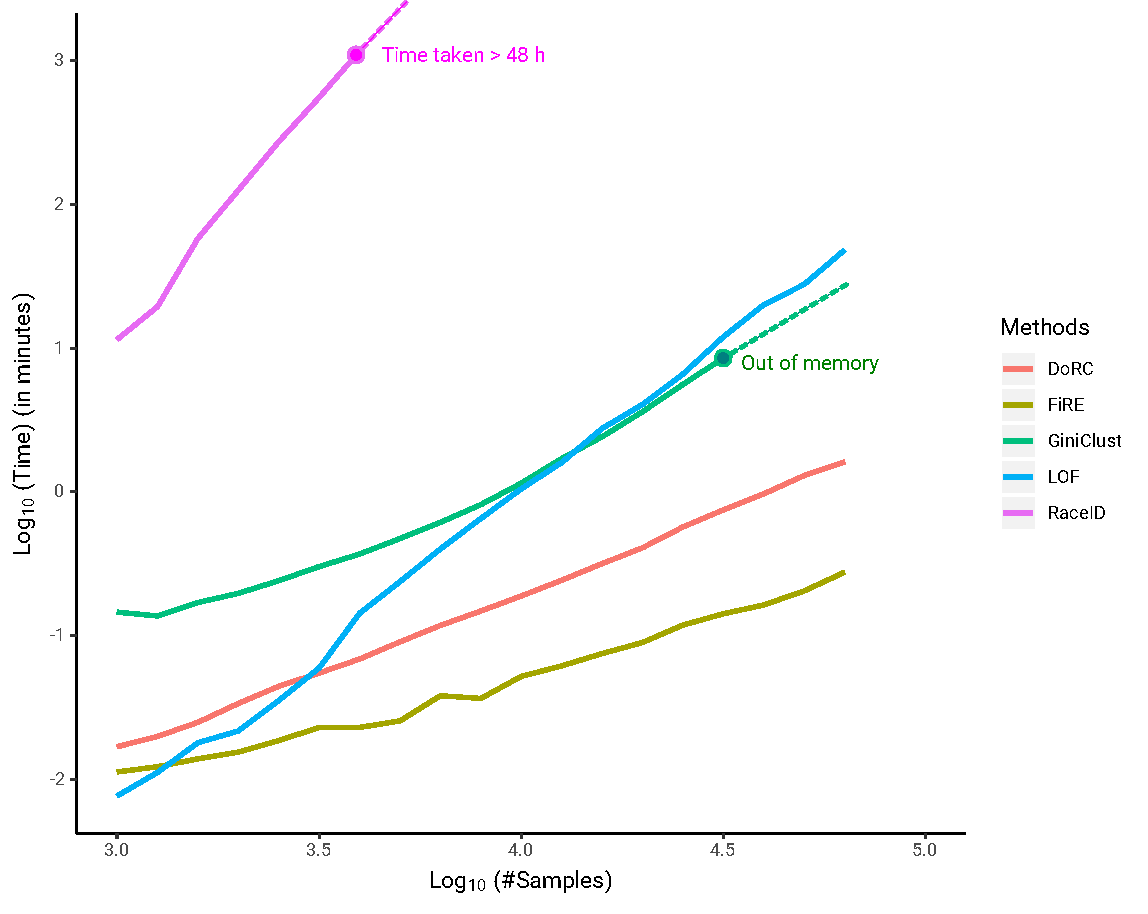
\includegraphics[width=0.9\textwidth]{Rplot_timecomplexity.pdf}
    \caption{DoRC is fast. Execution time is recorded for DoRC, FiRE, GiniClust, LOF and RaceID, while varying the number of cells from 1k
    to ${\sim} 68$k}
    \label{fig:timecomplexity}
\end{figure}

如图~\ref{fig:timecomplexity}所示,为了从~${\sim}68$k scRNA-seq数据中发现稀有细胞。 
GiniClust和~RaceID~要么耗时,要么耗内存;
LOF~对输入数据规模非常敏感;
然而,DoRC~和~FiRE~都是非常快的,因为它们只需要不到~2~分钟就可以完成任务。
与~DoRC~相比,FiRE~的速度明显更快。
然而,孤立森林可以很容易地使用并行计算~\cite{hariri2018batch}。
因此,我们认为~DoRC~的性能还有提升空间。

\subsection{讨论和结论}
近来,单细胞转录组学大大改善了我们对细胞表型性质的理解。
它还加速了新细胞类型的发现。
这些新的细胞类型大多是罕见的,因为显然一种丰富的细胞类型如果在很长一段时间内不被我们观察到是很不可能的。
一个真正稀有的细胞类型只有通过分析成千上万的细胞才能被发现。
虽然过去几年的技术进步使我们能够进行超高通量的单细胞测序,
稀有细胞检测的可扩展方法几乎不存在。
与~FiRE~方法类似,DoRC~试图用一种务实和适用的设计来填补这一空白。
最值得一提的是,DoRC~避免了使用聚类作为中间步骤。
因为典型的聚类技术不仅耗时,但也不可能一次性完全绘制复杂组织中的细胞类型。

DoRC~给每一个单独的表达图谱都给出了一个稀有度分数。
通过~IQR阈值,DoRC也可以像~RaceID~和~GiniClust~一样提供二元预测。
DoRC的核心是通过使用~Isolation Forest~作为核心算法实现的。
Isolation Forest~是机器学习中被广泛研究、应用得很广的一种无监督的异常点~(离群值)~检测方法。
每个细胞的稀有度用``异常点得分"来表示,对于每个给定的点在相应的高维空间中。
我们展示了~DoRC~在利用~${\sim}68$k~人血细胞单细胞表达谱划分人血树突状细胞亚型的表现。
这是通过我们提出的新颖有效的细胞聚类方法~RafClust~实现的,可以解决稀有细胞异质性的问题。
RafClust~方法可以应用于一般的单细胞转录组聚类。
此外,在其他两个模拟数据集上的实验显示~DoRC~可识别人工伪造的稀有细胞并且对细胞类型特征也很敏感。
我们还表明,DoRC~是可扩展的,而且速度很快。

其实,除了孤立森林外,最近在一些领域提出了这几种方法~\cite{aggarwal2015theoretical,zhao2019pyod,liu2019generative,weng2019multi}~也值得关注。
特别是当处理超大型~scRNA-seq~数据的稀有细胞发现。
据我们所知,DoRC~是首次将异常检测方法之一应用于稀有细胞的发现。
因此,我们相信~DoRC~在未来检测稀有细胞领域上对于生物学家来说是一个很有前途和潜力的工具。

\subsection{可重复性}
DoRC方法的~Python~实现代码可在以下网址获得~\url{https://github.com/chenxofhit/DoRC}。
其他代码和相关数据集根据用户的要求酌情提供。

% \subsection{鸣谢}
% 我们要感谢与印度理工学院~Aashi Jindal博士富有成效的讨论。
% 这项工作得到了国家自然科学基金资助~(No.61622213,No.61732009)~、111项目~(No.B18059)~和湖南省科技计划~(2018WK4001)~的部分支持。